%==============================================================================
% (c) David Molnar 2015
%==============================================================================

\chapter{Úvod}
Vyvíjet software v dnešní době není jednoduché. Konkurence na trzích je silná, požadavky na software se mění velice rychle a často je potřeba vydávat novou verzi aplikace co nejrychleji.

Za základní zásadu pro vývojový tým můžeme považovat Continuous Integration. Pomocí tohoto konceptu tým zůstane v synchronizaci a dokáže odstranit zpoždění způsobené integračními chybami. Je důležité si ale uvědomit, že Continous Integration je pouze prvním krokem k dosažení cíle. Další stanice je Continuous Delivery, tzn. nejenom častá integrace, ale i časté nasazení a uvolnění nové verze aplikace do produkce. Rozchodit nasazení ve smyslu Continuous Delivery není jednoduché, záleží to samozřejmě i na složitosti projektu. Nesmíme se ale zapomenout na okamžité výhody. Dlouhé, pracné a problematické vydávání verzí a jejich nasazení se stane věcí minulosti. Díky tomu zákazníci uvidí okamžitý pokrok vývoje objednaného produktu, který dodá funkcionalitu, kterou potřebují a využívají každý den. Je potřeba se zmínit i o výhodě, že tímto se také odstraní jeden u největších zdrojů stresu a napětí v týmu.

Velice inspirativní je projekt a tým vedený panem Kentem Beckem \cite{ContDelivery}. Tento velice disciplinovaný tým každý večer nasazoval novou verzi své aplikace přímo do produkce. Takový způsob implementace má několik výhod: napsaný a hotový kód neleží ve verzovacím systému\footnote{SVN, Git, TFS atd.} bez využití a tým dokáže velice rychle reagovat na problémy a na nové příležitosti. Navíc je zajímavý, že tento způsob práce vedlo k prohloubení vztahů mezi členy týmu a nárůstu důvěry zákazníka ve firmě. 

Continous Delivery dokáže snížit dobu trvání cyklu od první myšlenky a nápadu až do použitelný software. Myšlení ve smyslu Continuous Delivery upadlo na dlouhou dobu v zapomenutí, někde mezi vývojovým a nasazovacím týmem. Proto je velice důležité tyto dva týmy co nejvíce spojit. Nesmíme se zapomenout na to, že základem všeho je vysoká stupeň automatizace -- jednotlivé operace budou rychlé, opakovatelné, snadno testovatelné a kvalitní (bez chyb).

Našim hlavními průvodci v této práci budou Jez Humble a David Farley, průkopníci a známí aktivisti zásad Continous Delivery. Jejich kniha \cite{ContDelivery} bude pro nás sloužit jako Bible. 

Tato práce se detailně zabývá implementací zásad Continuous Delivery při urychlení vývoje a nasazení jedné ukázkové aplikace. Ukázkový projekt je webová aplikace s MSSQL databází. Dále obsahuje i jiné části, které budou popsané v kapitole \ref{ch:impl}. 

V kapitole \ref{ch:teorie} bude čtenář seznámen se základními pojmy z oblasti agilních metodik vývoje a doručení softwarových produktů. Kapitola \ref{ch:impl} se detailně zabývá návrhem a implementací ukázkové aplikace. Vzhledem k tomu, že je to ukázková aplikace, nebudou všechny detaily implementovány. V pokračování je popsán vývoj jednotlivých nástrojů a vytvoření infrastruktury (Active Directory domain, testovací prostředí atd.), kam bude aplikace nasazena. Vyhodnocení výsledků se uskuteční v kapitole \ref{ch:vyslekdy}. Pokusíme se porovnat výhody a nevýhody bez aplikování a pomocí Continous Delivery. V závěru v kapitole \ref{ch:zaver} bude následovat souhrn práce.

Naším cílem tedy bude ukázat, že je možný dodat vysoce kvalitní softwarový produkt velice často, třeba i denně a to bez zbytečných problémů a zádrhelů. Budeme k tomu používat hlavně Microsoft technologie.

V celé této práci budeme označovat pojmy Continous Delivery zkratkou CD a Continous Integration zkratkou CI. Ostatní zkratky jsou v tabulce zkratek na konci práce.

\chapter{Teoretická část}
\label{ch:teorie}
V této kapitole seznámíme čtenáře se základy Continous Delivery. Ukážeme, jaké problémy lze vyřešit pomocí tohoto konceptu. Budeme čerpat z knihy\cite{ContDelivery}.

\section{Deploymnet pipeline}
Ve vývoji software je velice důležitý, jakým způsobem bude vyvíjený produkt dodán uživateli. Jaká je rychlost, efektivita, spolehlivost a kvalita dodání. Většina vývojářů se soustředí na analýzu, psaní kódu a někteří i na testování (unit testy, integrační testy atd.).
Existuje spousta metodik pro vývoj software, většina z nich se ale  soustředí na zpracování požadavku a na jeho vliv na proces vývoje.

Nejdůležitější technikou pro nás bude tzv. deployment pipeline. Deployment pipeline je automatizovaná implementace procesu buildování, testování, nasazení naší aplikace. Samozřejmě každá organizace bude mít svoji vlastní implementaci, nicméně principy a zásady budou stejné. Příklad deployment pipeline-u je vidět na obrázku \ref{fig:pipeline}.

\begin{figure}[]
  \centering
  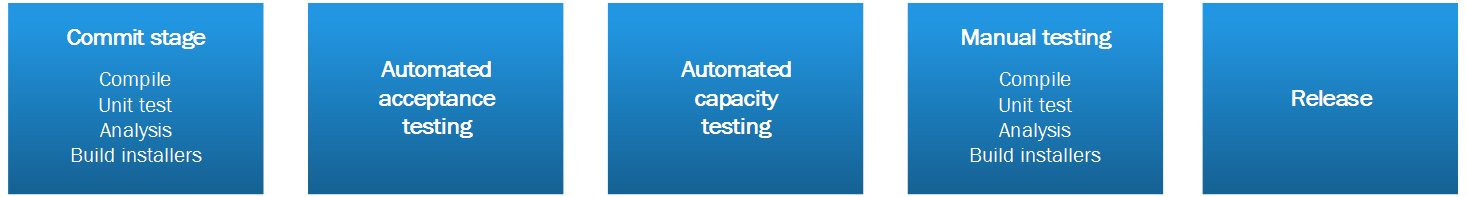
\includegraphics[width=15cm]{fig/pipeline_overview.png}
  \caption{Deployment pipeline overview}
  \label{fig:pipeline_overview}
\end{figure}

\begin{figure}[]
  \centering
  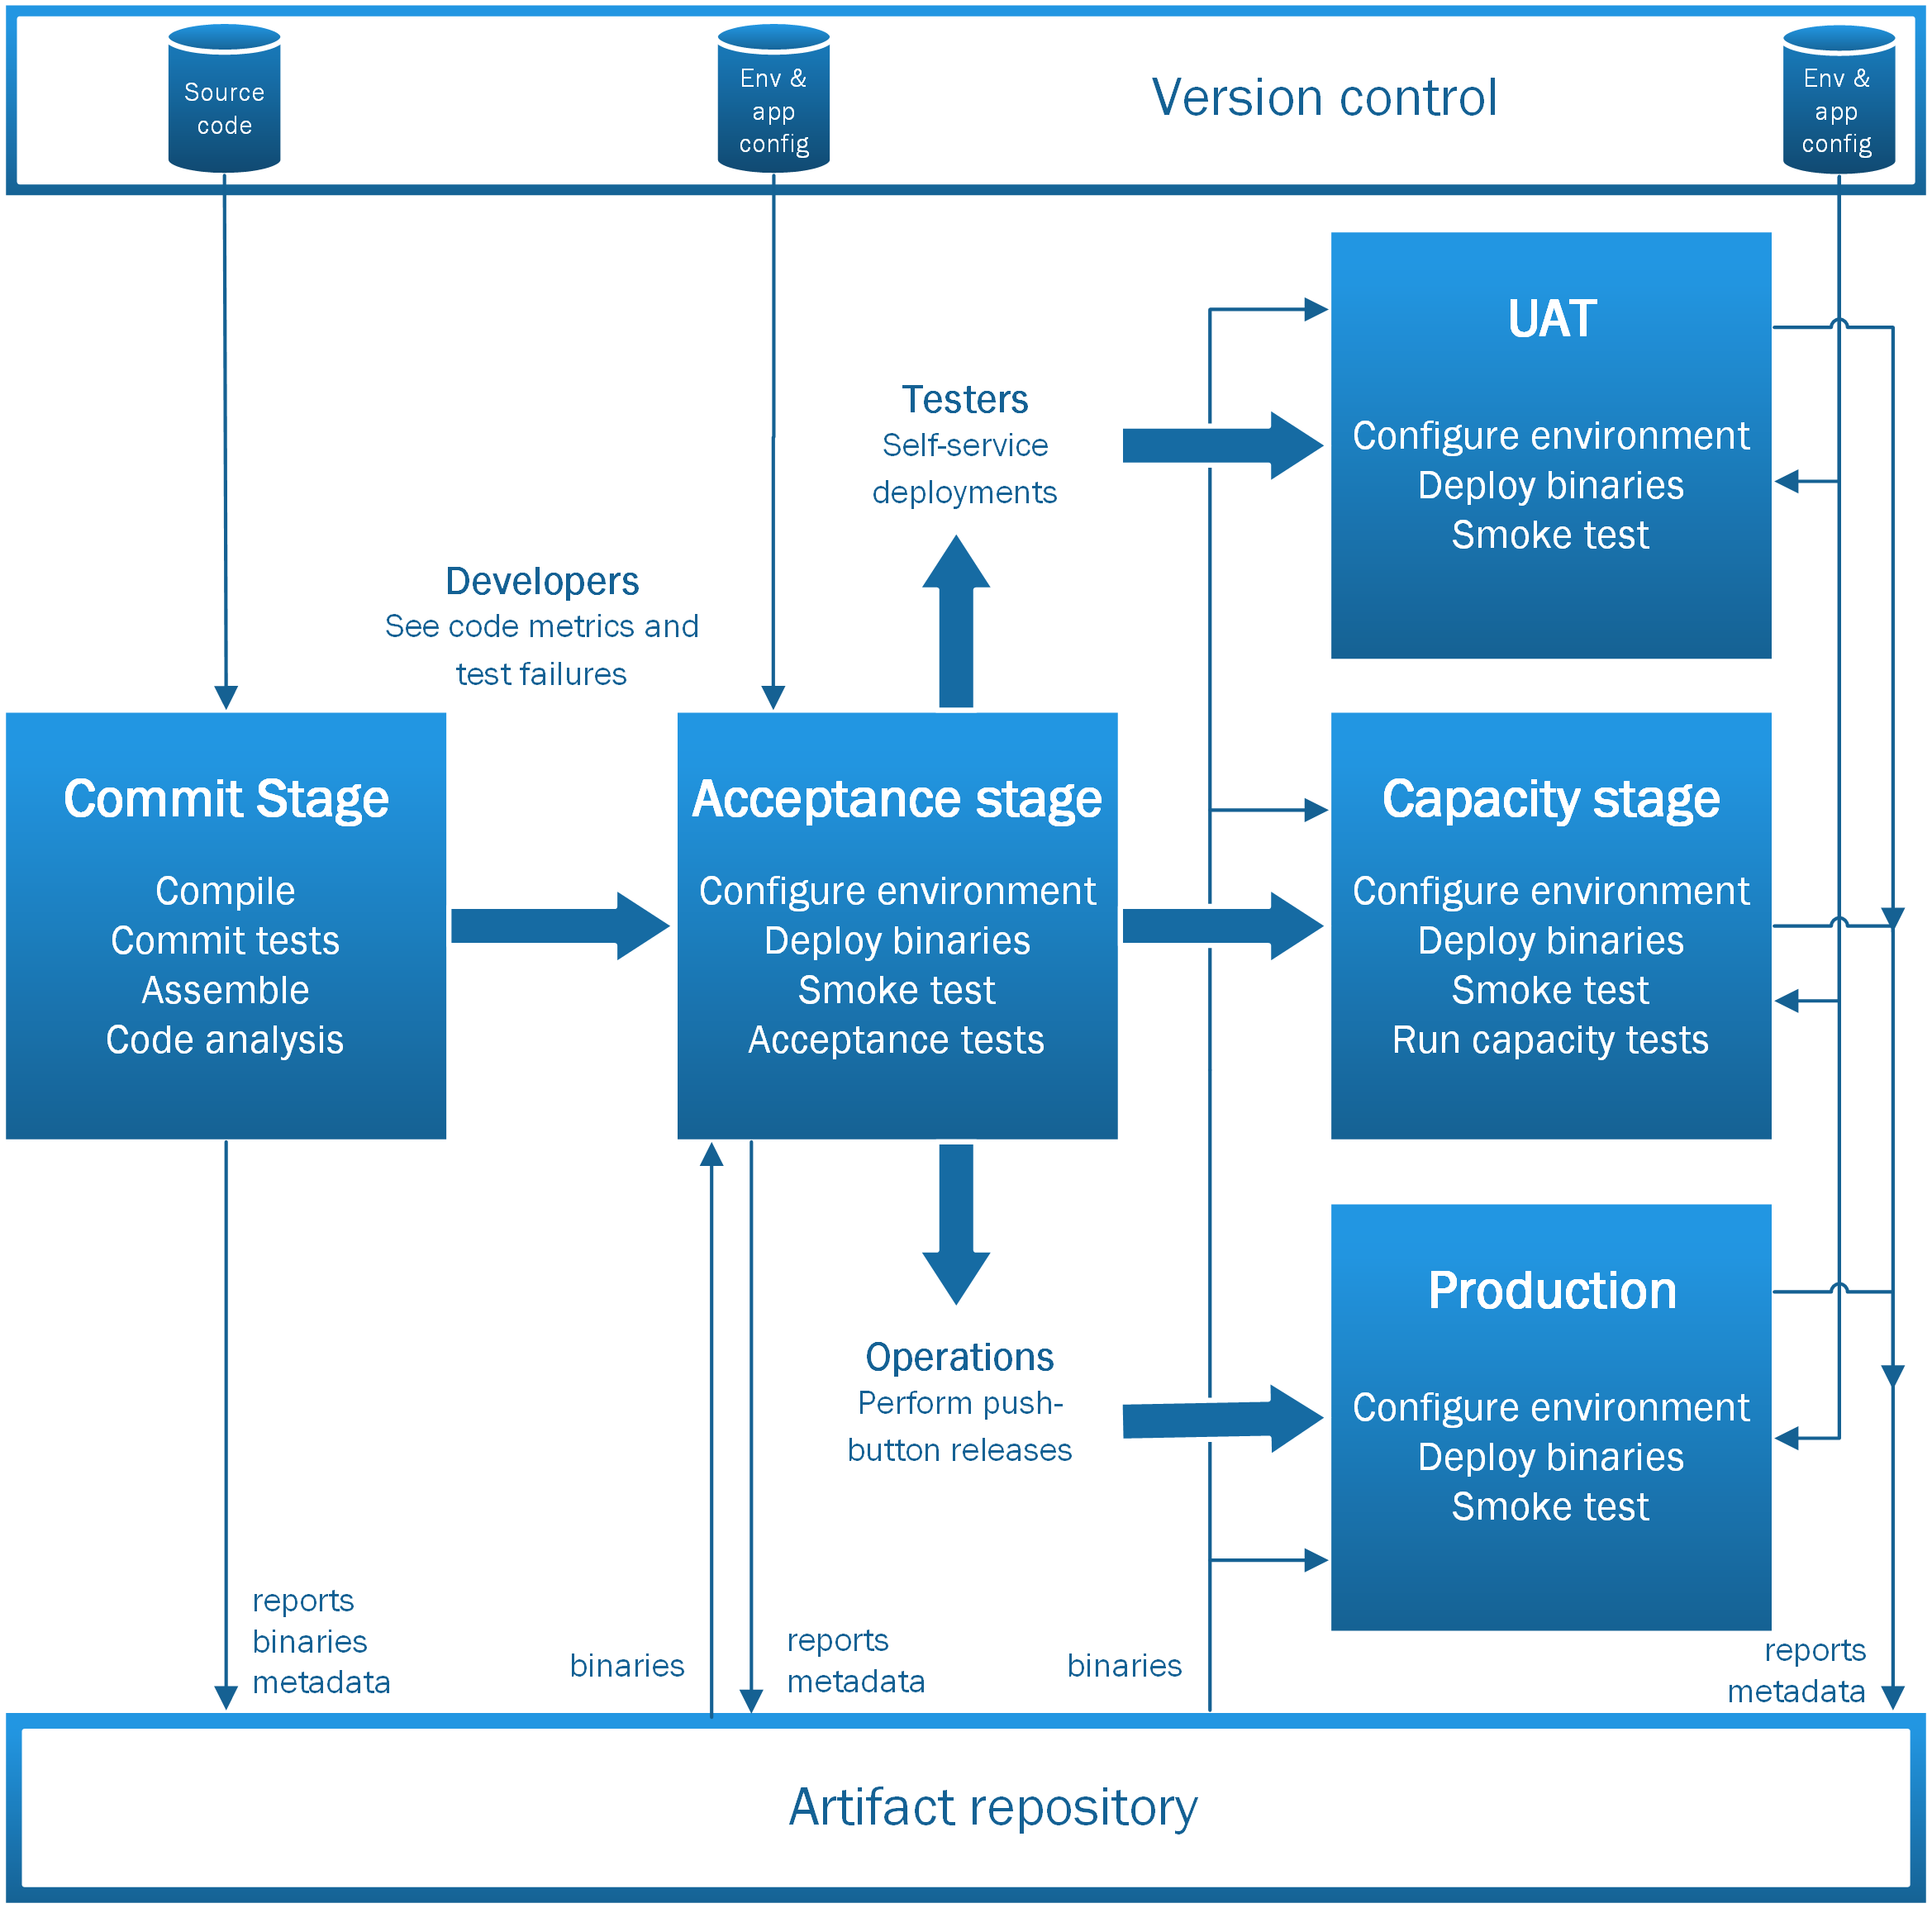
\includegraphics[width=15cm]{fig/pipeline_basic.png}
  \caption{Základní deployment pipeline}
  \label{fig:pipeline}
\end{figure}

\begin{figure}[]
  \centering
  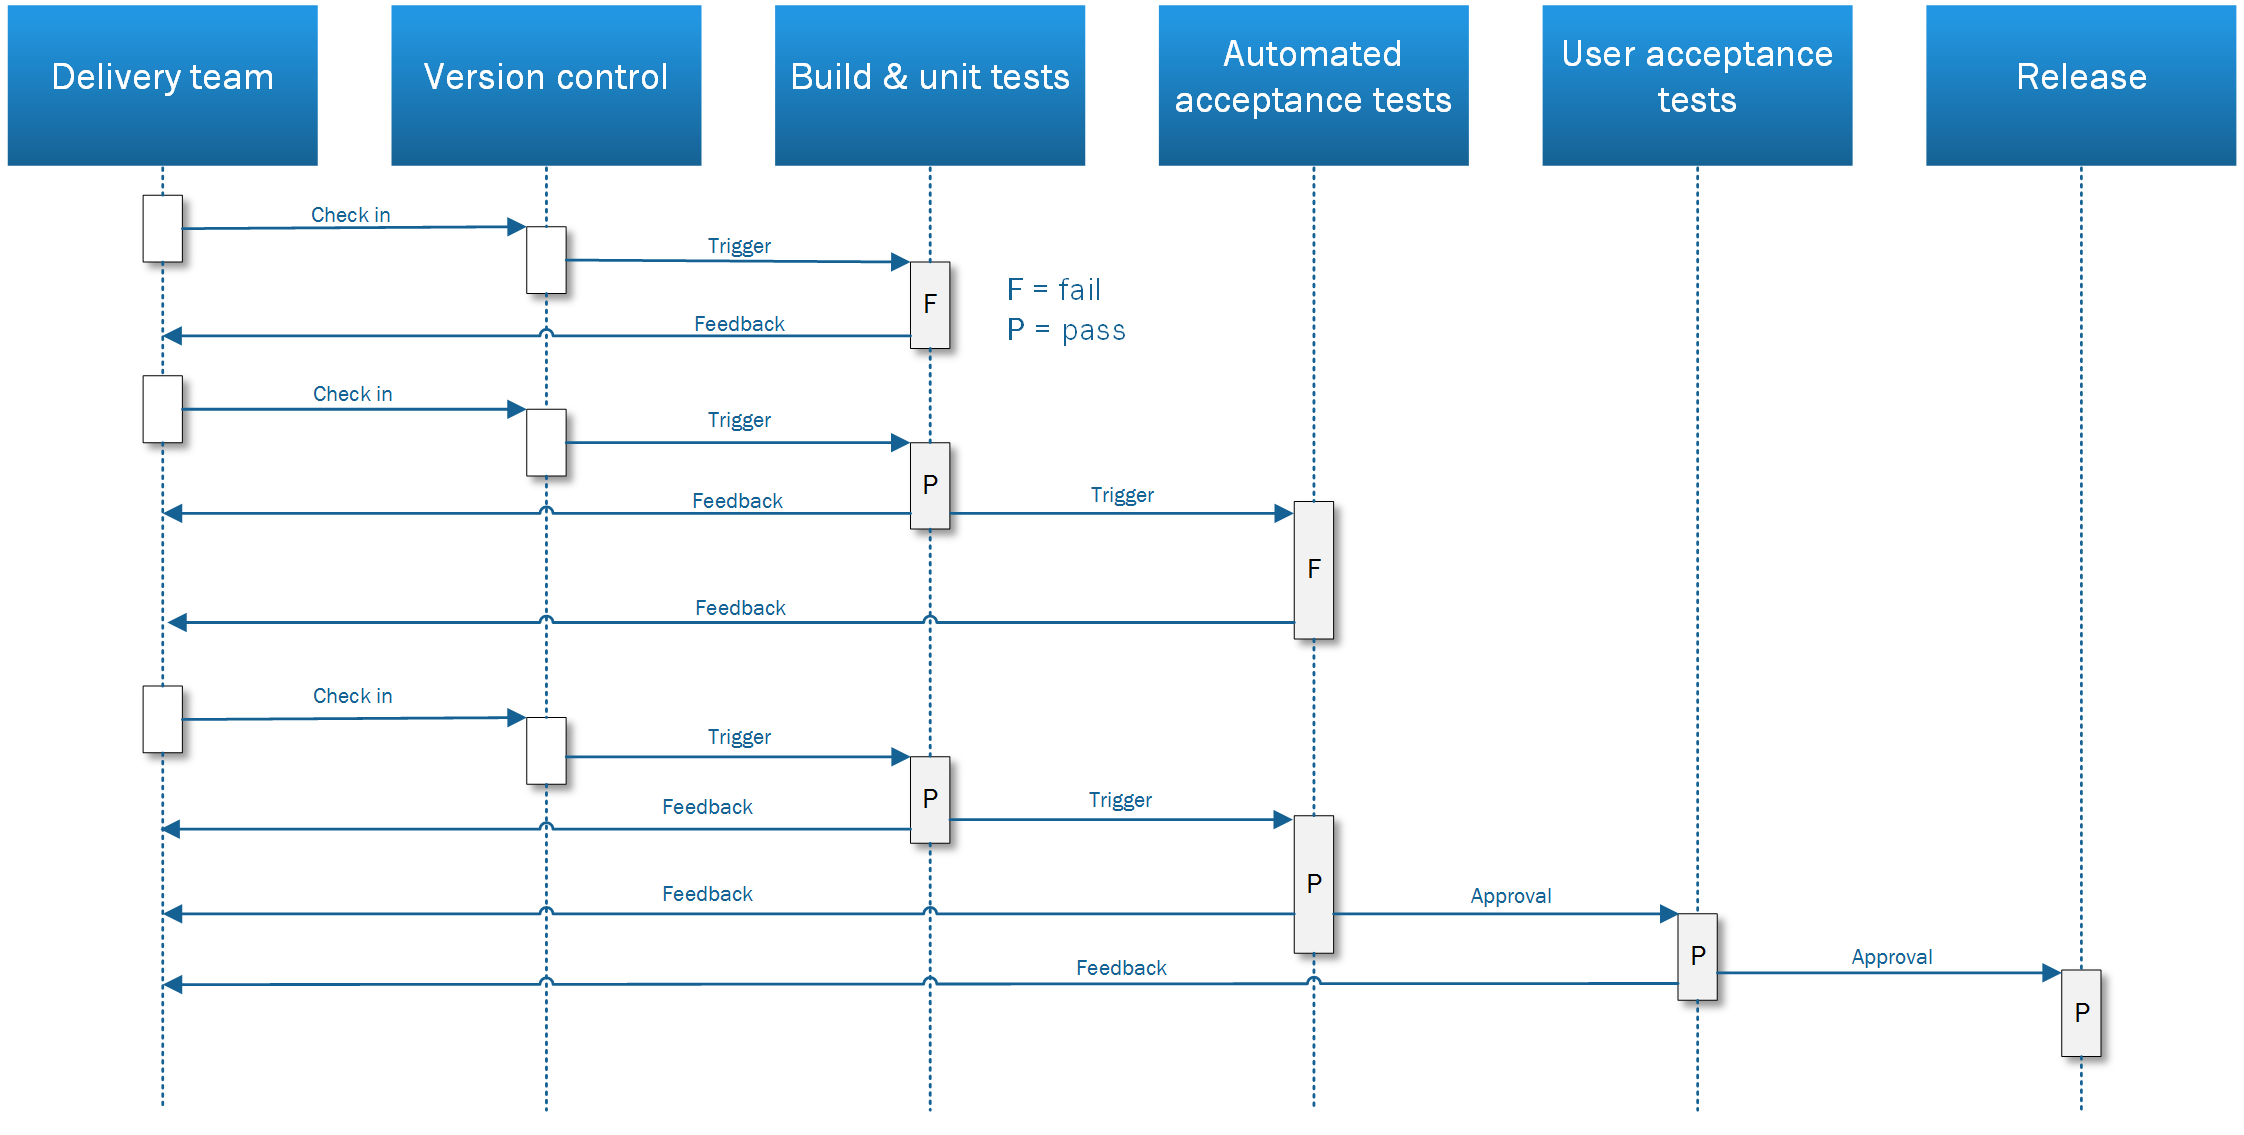
\includegraphics[width=15cm]{fig/pipeline_changes.png}
  \caption{Changes moving through deployment pipeline}
  \label{fig:pipeline_overview}
\end{figure}

Každá změna ve zdrojovém kódu, v konfiguraci nebo v prostředí způsobuje vytvoření nové instance pipeline-u. První krok je vytvoření binárek a installerů. Pak následuje testování, které ověří, jestli produkt má dostateční kvalitu. Každý test nám poskytne důvěru, že daná kombinace binárek, konfigurace a prostředí bude fungovat. Testování nemusí být vždy plně automatizovaný -- často je potřeba, aby člověk manuálně ověřoval výstupy. 

Největší výhodou deployment pipeline-u je, že zviditelní každou část vývojového procesu pro všechny členové týmu. Tým takto dokáže zajistit lepší kolaboraci. Další výhodou je i zlepšení zpětné vazby -- problémy jsou identifikovány a odstraněny co nejrychleji. Umožňuje i to, aby tým mohl nasazovat jakoukoli verzi softwaru kdykoli pomocí zcela automatizovaného procesu.

\section{Běžné antipatterny nasazování}
Krok nasazení u většiny moderních aplikací je procesem komplexním, zahrnujícím spoustu dílčích kroků. Mnoho organizací nasazuje software manuálně. Každý krok se provede manuálně, jako atomická operace. Všechna rozhodnutí, dělaná během nasazení, jsou náchylná k lidským chybám. Navíc jednotlivé kroky je možné udělat po každém trošku jinak, co může vést k různým nejasným a nekvalitním výsledkům.

\subsection{Manuální nasazování}
Tento bod může být charakterizován následovně:

\begin{itemize}
  \item Existuje velice detailní dokumentace, který popisuje proces nasazení
  \item Při ověření kvality se spoléhá především na manuální testování 
  \item Příliš časté dotazy na vývojový tým, ohledně vysvětlení chyb při nasazení
  \item Nasazovací proces se v průběhu vydání verze často modifikuje a opravuje
  \item Prostředí mají rozdílné konfigurace, např. aplikační servery s různými konfiguracemi aplikačního poolu, nekonzistentní struktury složek, různá verze prerekvizit atd.
  \item Nasazení a vydání verze trvá hodiny, občas i několik dnů
\end{itemize}

\subsection{Nasazení do produkce až po dokončení vývoje}
V tomto případě je aplikace nasazena do produkce až ve chvíli, kdy vývojový tým zcela dokončil vývoj. Charakterizace:

\begin{itemize}
  \item Jestliže aplikace byla testována, testeři testovali na vývojových stanicích
  \item Lidi z nasazovacího týmu uvidí novou verzi aplikace teprve během nasazení. V některých organizacích existují dva týmy: jeden pro nasazení do testovacího prostředí a jeden pro produkci. Vybudovat prostředí, které je podobné produkci, je velice drahé; přístup k němu je přísně kontrolované, případně je možné, že vůbec neexistuje.
  \item Vývojový tým sestaví binárky, instalátory, konfigurační soubory, databázové migrační skripty a nasazovací dokumentaci, které pak předá nasazovacímu týmu. Tento tým následně provede samotné nasazení -- většinou do prostředí, které předtím nebylo nikdy otestováno.  
  \item Kolaborace mezi vývojovými a nasazovacími týmy je slabé, nebo vůbec neexistuje. Lidé nechtějí zlepšit komunikaci, raději se spoléhají na dokumentaci atd.
\end{itemize}

Slabá spolupráce je pak kompenzována ad-hoc řešením: emaily, telefonní hovory, rychlé opravy. Přináší to stres, spěch a nízkou kvalitu. Disciplinovaný tým zahrne všechny informace o nasazení do nasazovacího plánu, ale i přesto je tento postup málokdy účinný. Většinou je potřeba dodat produkt v určitém termínu, což může vést k nárůstu tlaku mezi členy týmu a ke zhroucení předem definovaného postupu nasazení. 

V následujících kapitolách ukážeme, jak nám může pomoct integrování testovacích, nasazovacích činností do vývojového procesu. Budou to činnosti každodenní práce. Když přijde čas nasazení do produkce, riziko, že něco nefunguje, bude velice malé -- postupy již budou ověřeny a vyzkoušeny týmem mnohokrát v nejrůznějších prostředích. K tomu ovšem musí být zajištěna časná spolupráce všech lidí, podílejících se na vývoji a doručení.

\subsection{Manuální správa konfigurace produktivního prostředí}
Mnoho organizací spravuje konfigurace produktivních prostředí prostřednictvím speciálního týmu -- tzv. nasazovacího týmu. Pokud je potřeba udělat nějakou změnu, např. upravit parametry databázového připojení v connection stringu, zvýšit maximální povolenou velikost příchozího requestu na webovém serveru, pak potřebné akce provede tento tým zcela manuálně, přímo v produkci. Ve většině případů historie změn neexistuje, pokud ale ano, je to manuální záznam v databázi, na kterou se často zapomene.

\begin{itemize}
  \item Nasazení do testovacího prostředí bylo několikrát úspěšné, nasazení do produkce se přesto nezdaří.
  \item Nasazovací tým dlouhou dobu připravuje prostředí pro nasazení.
  \item Nelze udělat krok zpátky na dřívější konfiguraci systémů, mezi které patří operační systémy, aplikační, webové a databázové servery a jiné infrastrukturální nastavení.
  \item Produkční a jiné servery mají různá verze operačních systémů, aktualizací, knihoven a to zcela neúmyslně.
  \item Úprava konfigurace je provedena přímo na produkčních serverech, např. prostřednictvím RDP, SSH atd.
\end{itemize}

Všechny aspekty testovacích, produkčních a jiných prostředí, obzvlášť konfigurace aplikací třetích stran, by měli být uplatněny z verzovacího systému pomocí automatizovaného procesu. Klíčová věc je správa konfigurace, např. i to, že jsme schopni obnovit každou část infrastruktury používanou naší aplikací, tzn. operační systémy, aktualizace, konfigurace OS, knihovny třetích stran atd. 

Nejjednodušším způsobem, jak docílit automatizované konfiguraci, je virtualizace. Nemělo by docházet k manuálnímu provedení změn v testovacích ani v produkčních prostředích. Jediným způsobem by mělo být vytvořený automatizovaného procesu.

Vyvíjená aplikace často závisí na jiné aplikaci. Z toho důvodu je důležité, aby bylo možné rychle zobrazit verze aktuálně nasazované aplikace, operačního systému a aplikací třetích stran. Během většiny nasazení se dělají změny až po poslední chvíli. Musí existovat takový způsob zavádění změn, který je zaznamenáván a otestován. Tyto změny by pak měly být propagovány prostřednictvím automatizovaného procesu. V případě, že se nasazení nezdaří, mělo by být možné provedené změny nebo předchozí verzi aplikace vrátit.

\section{Jak dosáhnout cíle?}
Prvním klíčovým slovem je \textbf{automatizace}. V případě, že proces nasazení, testování a buildování není automatizován, pak není ani opakovatelný. Po každém se bude lišit kvůli změnám v konfiguraci aplikace, konfiguraci operačního systému a prostředí. 
Manuální kroky jsou náchylné k chybám a navíc není možné zpětně určit, co přesně bylo provedeno. Takovým způsobem nelze zaručit vysokou kvalitu výsledků. Vydání nové verze se velice často stává uměním. 

Další klíčovou vlastností je, aby proces byl prováděn \textbf{často}. Pokud nové verze vydáváme často, pak rozdíly mezi nimi budou malé. Pro nás to znamená, že nasazení lze snadno vrátit -- riziko je malé, protože jsme provedli málo změn. Časté nasazení vede i ke zlepšení zpětné vazby od zákazníka. Jeden z našich hlavních cílů je, dostat zpětnou vazbu co nejdříve. Kód, konfigurace, nastavení a funkcionalita, které nikdo předtím neviděl a jenom leží ve verzovacím systému, je rizikové -- může se nám zdát, že je vše v pořádku a překvapení přijde až po dlouho dobu, často ve formě supportních ticketů a nespokojených zákazníků.

\section{Hlavní výhody CD}
Hlavní výhodou zásad CD, které jsme popisovali v předchozí části je to, že vytváří proces, který je opakovatelný, spolehlivý a předvídatelný. Tyto vlastnosti vedou ke snížení doby cyklu vývoje, s tím naši uživatelé dostanou novou funkcionalitu a opravy chyb mnohem rychleji. Musíme si uvědomit, že může to znamenat nějakou investici, kterou ale rychle získáme zpátky.

\subsection{Posílení týmu}
Jednou z klíčových zásad CD je, že je to systém, který umožní testerům, nasazovacího týmu a lidem z podpory, aby aplikaci sami zprovoznili v libovolné verzi, do libovolného prostředí. Praxe ukázala, že doba trvání vývojového cyklu je ovlivněna i tím, že členové týmu čekají na nějakou dobrou verzi aplikace. Často to přináší nekonečnou emailovou komunikaci, založení supportních ticketů atd. Pomocí deployment pipelinu tento problém je zcela odstraněn. Každý má možnost vidět dostupné verze a po vybrání aplikace nasadit pouhým kliknutím na ikonku.

\subsection{Snížení počtu chyb}
Do dané aplikace se mohou dostat chyby z nejrůznějších míst. Uživatelé mohou požádat o nevhodnou věc. Analytik zachycující požadavek, pochopí to spatně. Vývojáři vytvoří ne úplně správně fungující až chybný kód. 
Aby naše aplikace fungovala, je potřeba zajistit spoustu věcí: správnou verzi zdrojového kódu, správnou verzi databázového schématu, správnou konfiguraci webového serveru, ale musí být nastaven třeba i správný URL na nějaký externí systém. Správa konfigurací znamená ovládání těchto informací, od prvního bitu až po poslední.

Nechme počítačům práci, v čem jsou opravdu dobré: správa zdrojového kódu, konfiguračních souborů, detekování změn, skripty pro vytvoření databází, schémata, konfigurace prostředí, operačních systémů atd. Takovým způsobem jsme schopni zajistit, aby všechno probíhalo tak, jak to daná aplikace vyžaduje.

\subsection{Snížení stresu}
Možná největší výhodou CD je snížení stresu všech stran, zúčastněných na vydání nové verze aplikace. Většina lidí, kteří již zažili blížící se termín odevzdání/zveřejnění aplikace mohou potvrdit, jak moc stresující tato zkutečnost může být. Samotný stres může znamenat zdroj problémů v našem procesu vývoje. Může vést ke vzniku problémů. Úpravy např. databáze, databázových schémat přímo na produkčních serverech jenom proto, abychom zprovoznili aplikaci, nejsou dobrou praxí. 
Tlak, který způsobuje takový stres, vede k použití rychlých hacků. Problém jako takový je to, že vydání nové verze aplikace není běžnou činností, ale velkou událostí.

\subsection{Flexibilita nasazení}
Nastartovat naši aplikaci v novém prostředí by mělo být jednoduchým úkolem. Ideálně to znamená vytvoření virtuálních strojů (např. ze šablony) a pak vytvoření konfigurace, která je unikátní pro toto prostředí. Dále můžeme použít náš automatizovaný proces. V prvním kroku připravit prerekvizity, v druhým nasadit vybranou verzi aplikace.

\subsection{Cvičení dělá mistra}
Můžeme říci, že každý tým, který používá CI nebo iterativní vývojové techniky, bude potřebovat nasadit aplikaci často. Nejlepší strategií je, používat stejné postupy, instalátory atd., které budeme používat v produkčních prostředích. Nesmíme mít rozlišnou strategii pro testovací a produkční prostředí, anebo speciální tým a postup. 

Takovým způsobem každý den ověříme, že naše aplikace a nasazovací proces funguje. Jediným případem, kdy můžeme udělat výjimky, jsou vývojové stanice. Vývojáři mohou potřebovat např. sestavit svoje vlastní binárky. Snažme se ale i v tomto případě použít co nejvíce procesů, které používáme v produkci.

\section{Zásady doručení software-u}
V této sekci shrneme nejvýznamnější zásady, beze kterých žádný nasazovací proces nemůže efektivně fungovati. 

\subsection{Opakovatelné a spolehlivé nasazení}
Vydání nové verze aplikace by mělo být snadné, jelikož jsme nasazení vyzkoušeli a otestovali miliónkrát předtím. Opakovatelnost a spolehlivost vycházejí ze dvou zásad: automatizovat téměř vše a udržovat zdrojové soubory, konfigurace, skripty atd. ve verzovacím systému.

Nasazení aplikace může být zcela automatizované. Konfigurace aplikace taky může být automatizované, všechny potřebné informace uložené ve verzovacím systému. Je jasné, že fyzický hardware nemůže být ve verzovacím systému, ale virtualizace může významně pomoct.

\subsection{Automatizování téměř všeho}
Určitě existují věci, které není možné automatizovat. Jako příklady se dají uvést explorativní testování, kontrola některých výstupů a schválení nasazení. Některé typy nasazení, např. nasazení do produkčních prostředí, mohou vyžadovat schválení vedoucího. Musíme si ale uvědomit, že automatizace je možné ve více případech, než si na první pohled myslíme. Existují případy, kdy automatizace je extrémně náročná. Pro tyto případy je dobrou radou, že je lze vyřešit až na konci, nebo nevyřešit vůbec a najít jinou alternativní řešení. 

\subsection{Všechno je ve verzovacím systému}
Všechno, co je potřeba k sestavení, nasazení a testovaní aplikace, musí být ve verzovacím systému. Sem patří i specifikační dokumenty, testovací skripty, automatizované test cases, skripty ke konfiguraci, databázové skripty, knihovny, různé nástroje, technické dokumentace atd.
Je potřeba umožnit pro komukoliv, kdo se sedne k jedné ze stanic, aby mohl stáhnout aktuální verzi aplikace, následně provedl build a pak nasazení aplikace do libovolného prostředí. Dále je potřeba, aby aktuálně nasazená verzi bylo možné jednoduše identifikovat.

\subsection{Provádět často}
Tato zásada je z výše uvedených zásad nejobecnějším. Můžeme ji považovat spíš jako heuristiku. Integrace různých části velké aplikace je problematické, je to bolestivým procesem. Proto je důležité integrovat každý jediný commit/změnu ve verzovacím systému. Pokud např. otestování nové verze aplikace je časově náročné a neefektivním procesem, musíme to dělat častěji, třeba i každý den. To bude mít následek, že tým postupně vylepší daný proces a odstraní problémy.

\subsection{Zabudování kvality}
Opravit chybu v produkční aplikaci je velice drahé. Opravit tu stejnou chybu v testovacím prostředí je mnohem levnější. V ideálním případě by chyby měli být zachyceny ještě před komitnutím do verzovacího systému. Proto je důležité aplikovat ty zásady, které popisujeme. Pomohou totiž zachytit chyby co nejdříve.

Testování nesmí být považováno jako fáze následující po dokončení vývoje. Pokud testování necháme až na konec, tak to je již pozdě. Nebude dostatek času na opravování chyb a odstranění problémů. Navíc, uvědomujme si, že testování není doména jenom testerů, ale za kvalitu ručí celý tým jako celek, tzn. každý člen týmu.

\subsection{Hotové znamená nasazeno}
Pojem \uv{hotové} pro většinu vývojových týmu znamená, že daná funkcionalita je vyvinutá. Neznamená to ovšem, že zákazník funkcionalitu již viděl a již vůbec ne to, že nová verze aplikace s funkcionalitou je již nasazena. 

Nejlepší je, pokud pojem \uv{hotové} znamená následující: funkcionalita je hotová, pokud byla uživatelům úspěšně demonstrována v takovém prostředí, které je podobné produkčnímu. 

\subsection{Každý je zodpovědný za nasazení}
V ideálním případě, každý člen týmu vykonává svoji práci v prospěch týmu. Tým nakonec dosáhne úspěch nebo selže společně, jako tým a ne jednotlivce. Bohužel ale realita ve většině případu je jiná. Vývojáři hážou svoji hotovou práci na testeři, testeři dále na nasazovací tým. Pokud něco nefunguje, selhává, pak tým tráví víc času obviňováním, než opravou. Proto je velice důležité odstranit bariéry mezi těmito týmy. Někdy může stačit reorganizovat kancelář, aby tyto týmu byly blíž k sobě.

\subsection{Neustálé zlepšování}
Je potřeba zdůrazňovat, že nasazovací proces není statický, vyvíjí se spolu s aplikací. Tým by měl regulárně revidovat nasazovací proces a prodiskutovat, jaké zlepšení se v následující době uplatní.

\section{Rozdíly mezi Continous Integration/Delivery/Deployment}
TODO ?

\section{Technologie a nástroje}
V této sekci popíšeme některé nástroje a technologie, které budeme používat. ???

\subsection{Windows Server}

\subsection{IIS}

\subsection{Microsoft SQL Server}

\subsection{TeamCity}

\subsection{SCM}

\subsection{.NET Framework}


\chapter{Praktická část}
\label{ch:impl}
V této kapitole se budeme zabývat s konkrétní implementací zásad CD. Začínáme specifikací a návrhem jedné ukázkové aplikace, kterou pak budeme nasazovat. Součástí bude i vybudování a správa testovacího a produkčního prostředí. S podpůrnými technologiemi se seznámíme v kapitole analýzy a implementace.

\section{Specifikace}
Tady budou specifikace...

\begin{figure}[]
  \centering
  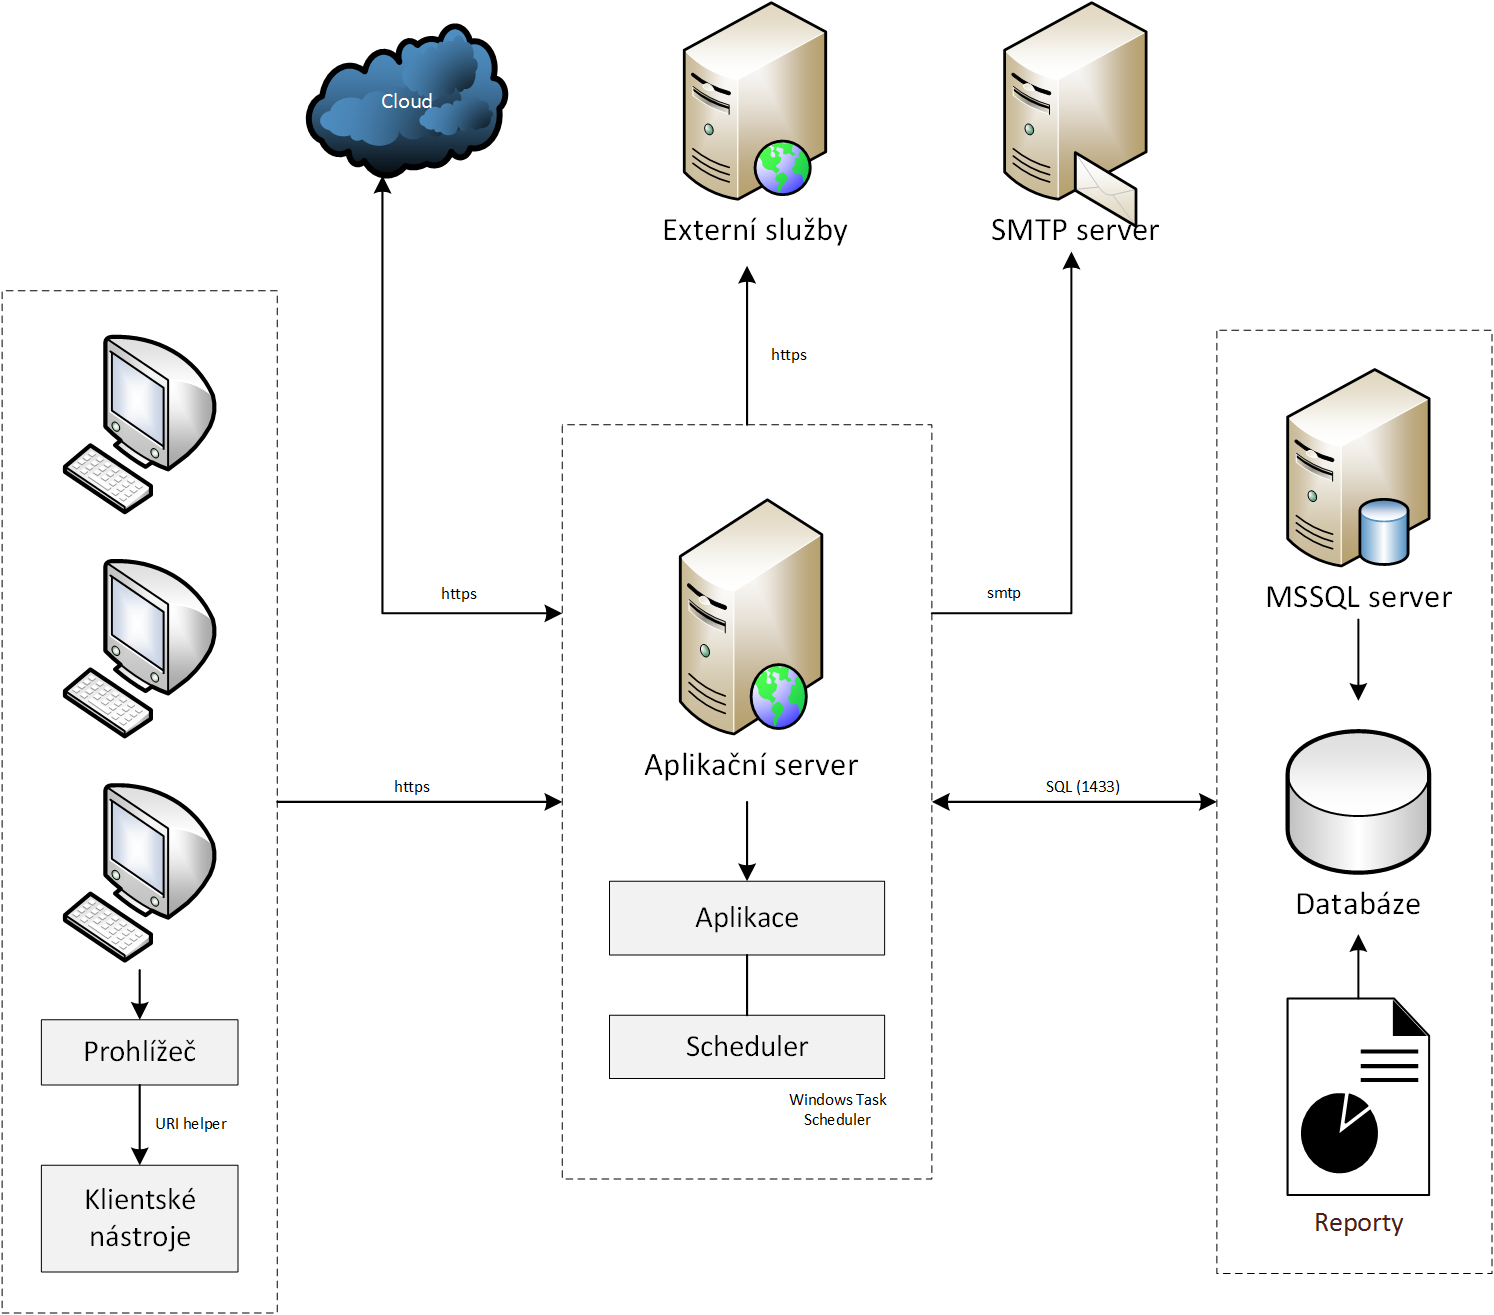
\includegraphics[height=10cm]{fig/app_architektura.png}
  \caption{Architektura ukázkové aplikace}
  \label{fig:architektura}
\end{figure}

\section{Analýza}
Tady bude analýza

\section{Implementace}
Tady bude popis implementace, vybrané technologie a SW, zajímavé části kódu, vytvořené nástroje a prostředí atd.

Nástroje pro
\begin{itemize}
  \item konfigurace, parametre, nastavení + GUI
  \item nasazovaní webu
  \item konfigurace IIS
  \item nasazovaní/vytvoření databáze
  \item aktualizace databázového schématu
  \item nasazení reportů (Report Server)
  \item nasazení Schedulerů, použití Windows Task Scheduler
  \item nasazení prerekvizit (.Net Framework, ...)
  \item nastartování a údržba virtuálních prostředí
  \item nástroje pro autentizace a předávání hesel (Windows, NTLM atd.)
  \item deploy a výběr certifikátů
  \item nástroje pro vývojáře: kopírování db, výběr prostředí, aplikování konfigů
  \item install/system center
  \item nástroje pro UI testování (Silverlight, HTML)
  \item maintenance mód a podpora blue/green
  \item instalace, konfigurace OS a virtuálních počítačů
  \item deployment pipeline v TeamCity  
  \item ...
\end{itemize}

\chapter{Vyhodnocení výsledků}
\label{ch:vyslekdy}
V této kapitole se pokusíme vyhodnotit výsledky práce z předchozích kapitol. Budeme porovnávat nasazovací proces nejdříve bez, pak pomocí zásad Continous Delivery. 

\section{Nasazení bez CD}
Co to znamená, jak to vypadá, kolik to trvá. Jaké kroky, problémy, náchylnost k chybám...

\subsection{Popis}
Podrobný popis situace...

\subsection{Výhody, nevýhody}
Výhody jsou...
Nevýhody jsou...

\section{Nasazení pomocí CD}
Zavedli jsme zásady CD, jaké změny jsme uplatnili, v čem je to lepší, kolik to stálo, ...

\subsection{Popis}
Podrobný popis situace...

\subsection{Výhody, nevýhody}
Výhody jsou...
Nevýhody jsou...


\chapter{Závěr}
\label{ch:zaver}
Závěrem bude krátké shrnutí naší práce. Podařilo se to a to, nepodařilo se ....

%=========================================================================
